\chapter {Introduction}

In the traditional Internet architecture, a single server handles multiple simultaneous incoming client requests.  
The bottleneck in such systems under high load can become lack of bandwidth from the server \cite{coopnet}, because bandwidth is split $N$ 
ways among the requesting clients (Fig. \ref{fig:traditional_http}).  When an increasing number of clients request a web page, that page 
therefore loads more and more slowly for users.  This problem occurs any time the ratio of bandwidth to clients is low, for example, when a server 
is poorly provisioned, it experiences a sudden spike in load, or a small number of incoming clients download very large files.  An example of this problem 
is the ``slashdot" effect, in which a sudden flash crowd of clients suddenly requests certain pages, overwhelming unexpectant servers.  
These situations cause web servers to server files slowly, become overwhelmed, or even crash.

This problem is commonly combated by distributing the requests among a set of servers that mirror the content of the original server (Fig. \ref{fig:server_only}).  
A company establishes a content distribution network (CDN) of mirrors by locating a set of servers in many different places on the Internet, then automatically redirecting clients to these servers, thus 
distributing the load to provide better performance.  An example of this is the large commercial CDN run by Akamai \cite{akamai}, which performs distributed
downloads for its clients.  For example Apple uses Akamai's CDN to distribute their iTunes\texttrademark   program.  This solution,  however, requires a dedicated pool of 
servers to provide the extra bandwidth.  Not all sites can afford a CDN, and  mirrors require cooperation, configuration, and maintenance.

As a cheaper alternative, many web sites are beginning to use \emph{peer-to-peer content distribution}, or \emph{swarming}, with BitTorrent.  In BitTorrent, clients 
download only some blocks of a file from a central server, and download the other blocks from their peers in the system.  While a client participates, it is both downloading 
the  blocks it needs and uploading the blocks it has to other peers (Fig. \ref{fig:normal_swarm}).  Peer-to-peer content distribution enables a 
web server to serve a large file to a large numbers of users with better scalability \cite{zappala}. Swarming protocols have been shown to actually decrease total download 
time per peer as the number of peers increases, which is the opposite of the traditional client-server paradigm \cite{slurpie}. 

\begin{figure}
  \subfigure[Traditional HTTP download]{
   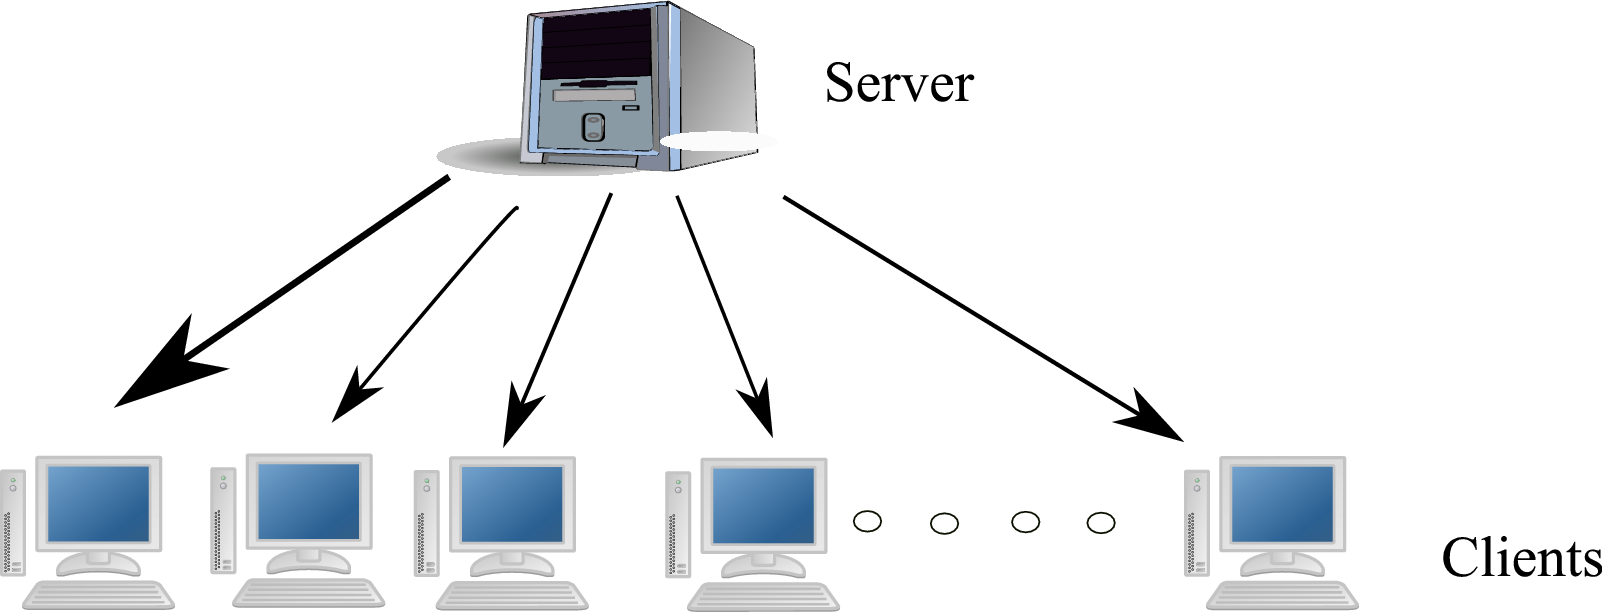
\includegraphics[width=9cm]{description_pics/traditional_http.png}
   \label{fig:traditional_http}
  }
\subfigure[Server CDN example]{
  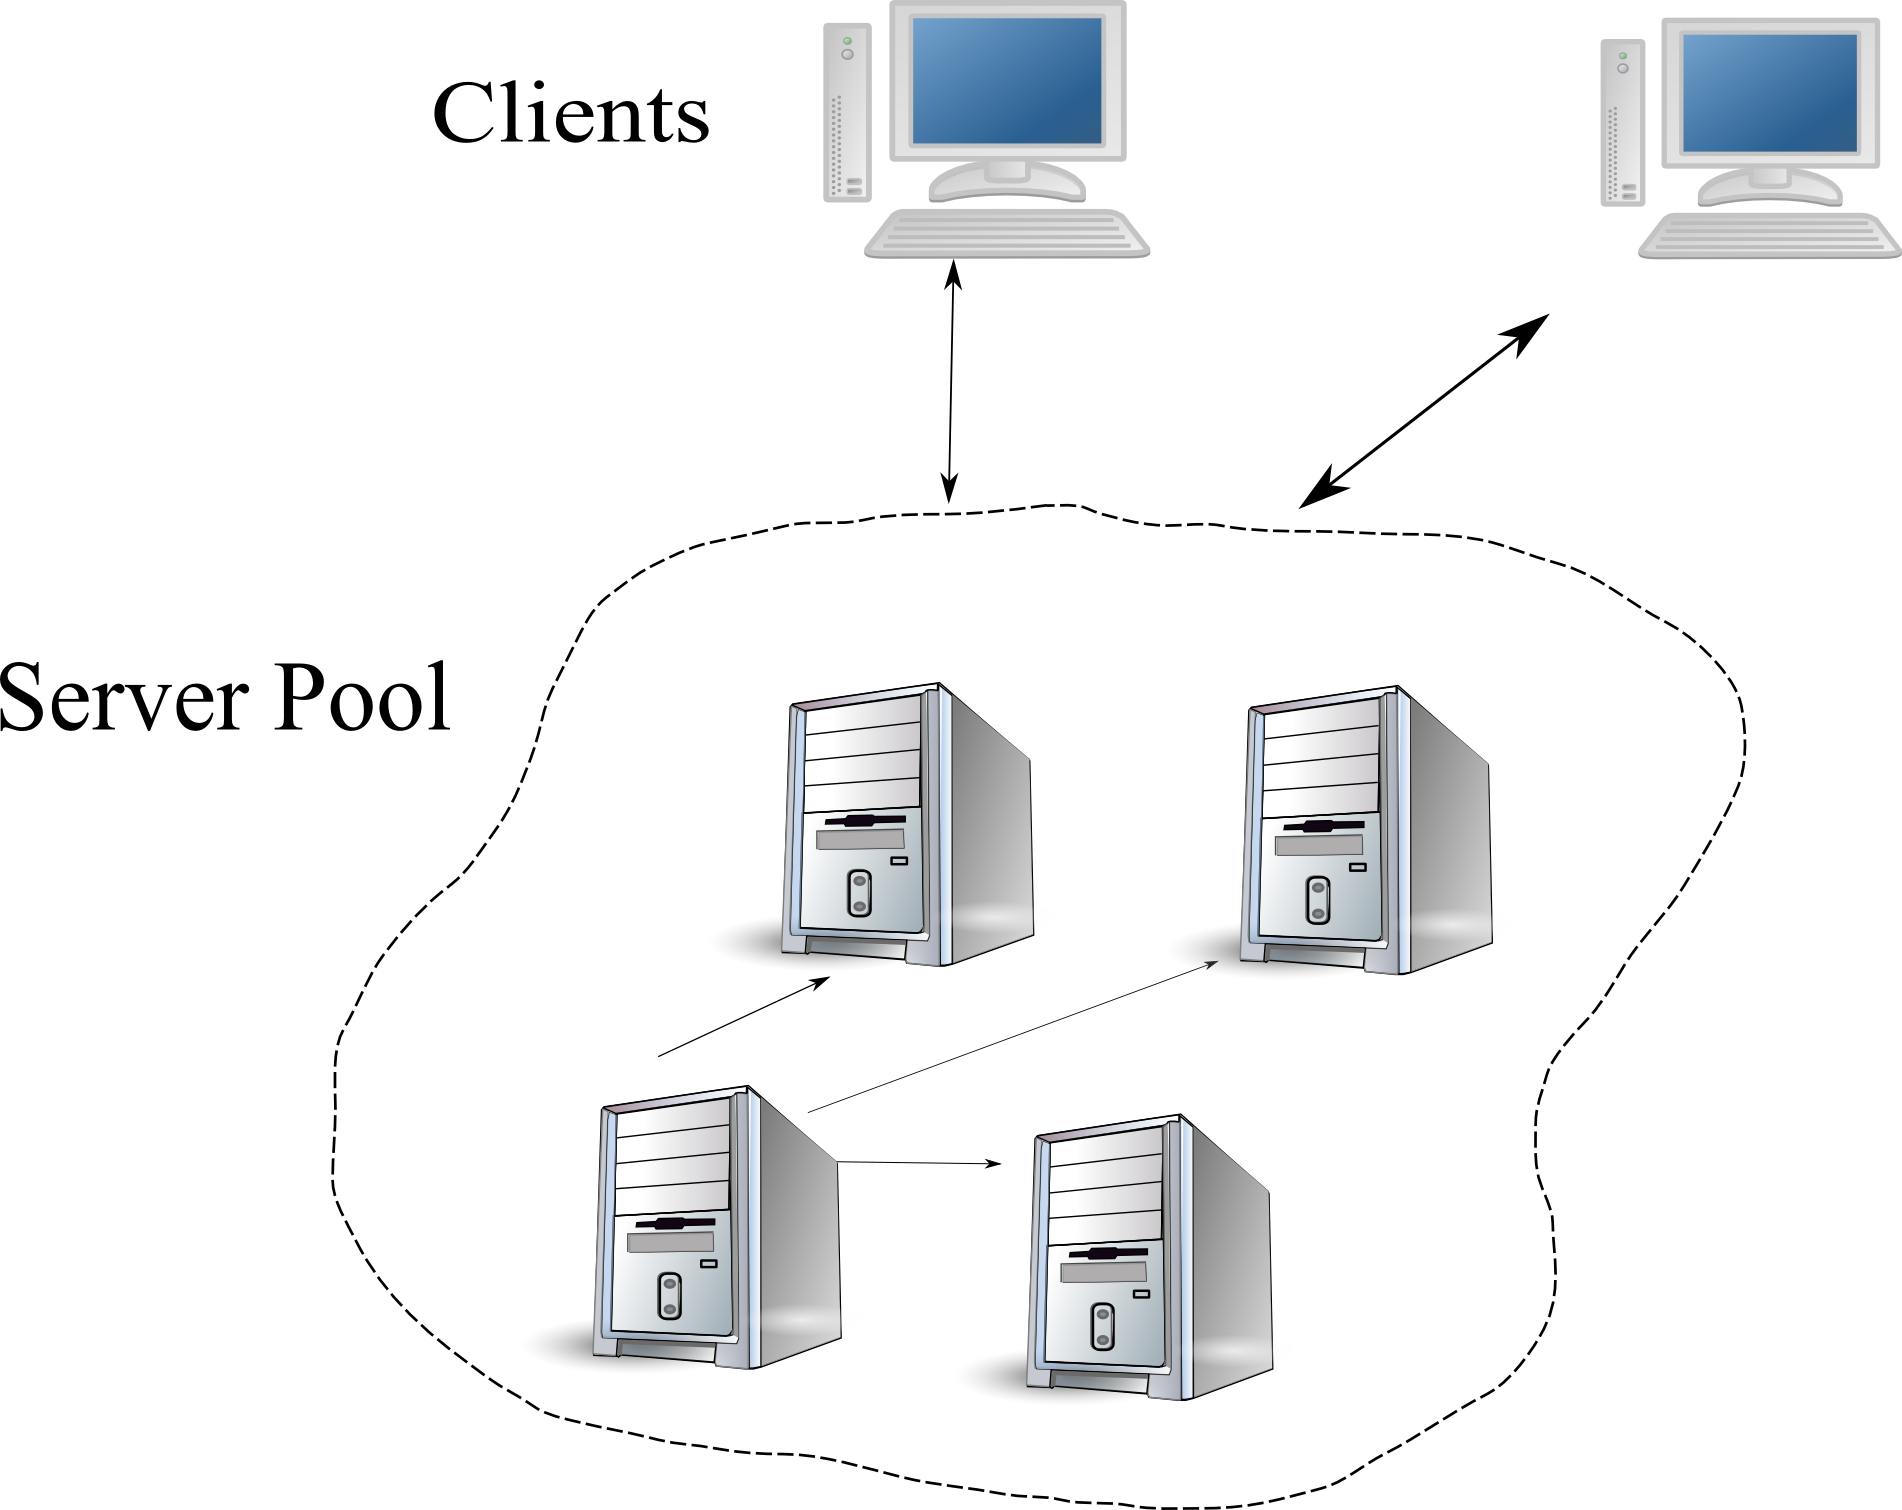
\includegraphics[width=8cm]{description_pics/server_side_only.png}
  \label{fig:server_only}
  }
  \caption{Traditional client server download}
\end{figure}

\begin{figure}
 \centering
 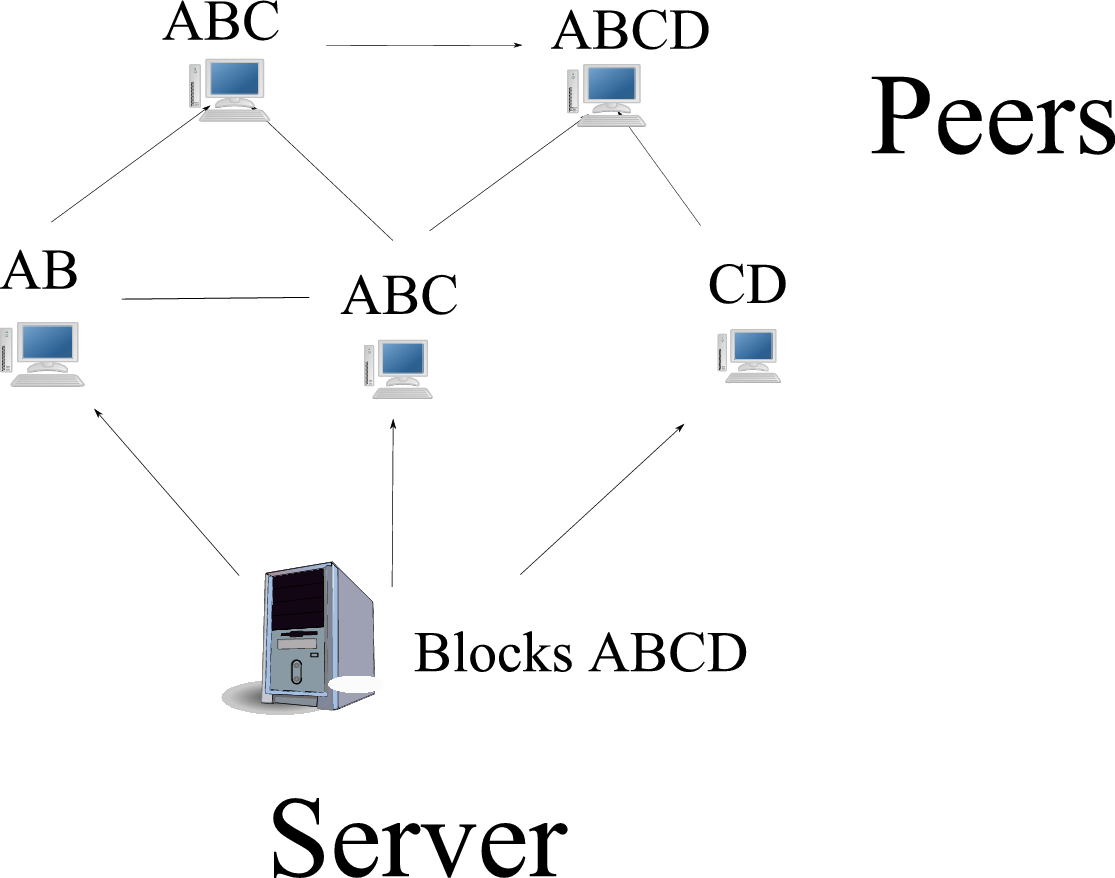
\includegraphics[width=8cm]{description_pics/normal_swarm.png}
 \caption{Swarming example.  Arrows represent block exchanges.}
 \label{fig:normal_swarm}
\end{figure}

Using BitTorrent currently requires some configuration for both servers and clients, and isn't well-integrated into normal HTTP downloads.  A server wishing to use BitTorrent 
must first create a special file with a ``.torrent'' extension that lists a target file's size, the MD5 hashes for each block of the file, and 
the IP address of a tracker for that file.  The tracker is a dedicated machine that helps connect the peers to each another, and must be administered
by the site using BitTorrent.  Users start a BitTorrent download by selecting the ``.torrent'' file on a web server, which launches a BitTorrent client program.
The BitTorrent client will contact the tracker to receive a list of peers who are currently downloading the file.  It then establishes connections and 
begins sharing and receiving blocks with its neighbors.

%->final ?:BitTorrent, for the download of the last block of a file, uses a kind of 'many peers downloading the same blocks.  It requests the last block simultaneously from many peers, so that if one peer is transmitting it very slowly, they will be quickly passed by one of the faster seeds, and thus download it quickly.

BitTorrent is not commonly used for serving all the files of a web site since it requires per-file configuration, and a tracker must be established for the files.  It is used mostly for large files where
configuration time is not as much of an issue.  Since BitTorrent uses a separate program, it will not work well for downloading web pages which must be viewed in a browser.  
BitTorrent also requires users to install client software and understand how and when to use it, creating a barrier to entry.  For example, many download sites offer links to BitTorrent downloads,
but users may ignore them.

In this thesis, we integrate peer-to-peer delivery into a standard web client, so that an unmodified web server can automatically offload traffic as load increases. 
This system provides for automatic integration of swarming downloads with HTTP, thus lessening the configuration and manual intervention needed for use.
Using experiments on PlanetLab, we show that peers who request small files can receive them at a rate of up to 30x the speed of traditional file server download, and
can decrease the load on busy servers.  

\chapter{Related Work}
Much work has been done to study distributed file downloading.  Solutions fall into three basic categories: client-side protocols, cooperative (client and server-side) protocols, 
and server-side protocols.

\section{Client-Side Protocols}
Protocols that use only client-side interaction require no change in the server software, allowing them to be implemented in clients without requiring servers to be aware of the changes.  However, this requires that clients must self-organize without the help of the centralized server.  Our protocol is an example of such a system.

Shared web caches are an example of a client-side only protocol.  They allow peers to download files from some well known cache -- typically a specific set of computers, such as those run by PlanetLab.  Coral \cite{coral} and CoDeen \cite{codeen} are examples of such caches.  Shared caches like these require a dedicated set of proxies, however.  
Squirrel \cite{squirrel} is another instance of a shared web cache.  Squirrel clients join a local Distributed Hash Table (DHT) 
which is used to track which files have been downloaded by which peers.  
The DHT is then used to locate the peer owners of files, who then serve as proxies for that file.  
The advantage of this is it doesn't require dedicated infrastructure.  
The disadvantage is it does not offer an algorithm for transparent transition to peer-to-peer delivery, nor does it allow for partial file downloads.  It was also built on the assumption of being run on a local (well-connected) network, not on the Internet at large.

Coral-style caches are useful, but have limitations.  They are constrained to the number of participants, and they require an infrastructure of hosts who are willing to altruistically provide bandwidth, which is rare, because of expense.  Also, when load surpasses the bandwidth of the 
combined sum of proxies, they will still become overburdened.  For example, if Coral receives a request for a file too many times, it begins redirecting peers back to the origin server, thus not solving the original problem.  
Coral is also limited in the size of files it can cache by PlanetLab policies.  With our system this should not be a problem, as more peers means that more are available to upload.  These systems also lack an algorithm for transition to peer-to-peer delivery, and sharing of blocks among peers.  They also add an extra hop in network latency per request, even if a request from the origin server would have been the fastest way to download the file.    

%The effect of  flash crowds can also be alleviated by searching among a random subset of Internet peers for desired files.  PROOFS \cite{proofs} (P2P Randomized Overlays to Obviate Flash-crowd Symptoms) uses flooded search to allow peers to locate 'popular' or 'flash crowded' files from other peers who have previously downloaded the same.  The creators conjecture that files that are the subjects of a flash crowd are likely to be locatable among random sets of peers, since they are popular, hence their use of a random flood search.  The benefit of this system is that nodes need not maintain a structured search system (such as a DHT). However, not having a DHT for lookup makes searches more random and slightly less accurate, with potentially higher overhead.  PROOFS also does not include parallel downloads nor offer a protocol for automatic transition to a peer-to-peer solution.

\section{Cooperative Protocols}

With cooperative protocols, a server and clients work together to provide scalable downloads.  Participation by the server makes it easier to build a system,
but it will only work for those sites that adopt the new mechanism.  

One style of cooperation for web servers uses redirection.  For web redirection, servers typically redirect clients to former clients that have downloaded files previously \cite{pseudoserving, coopnet}.  This allows a server to ``meter'' its upload speeds and redirect peers, when appropriate, thus providing a backup strategy for over-loaded servers.  An example of this is the pseudo-server system \cite{pseudoserving}.  This style of protocol typically requires changes to both the server and client software, however, and the server could still become overloaded in extreme cases.

A second style of cooperation uses swarming to download large files.  This is best exemplified by BitTorrent.  Swarming protocols are highly effective at serving loads orders of magnitude higher than an ordinary web server \cite{zappala}.

OnionNetworks has proposed an extension to HTTP to incorporate swarming.  With this protocol, HTTP response messages include hashes of files and a list of peers that clients
may connect to and download from in a swarming fashion \cite{onion}.  Unfortunately their proposal has not seen wide-spread adoptance nor research, and in extreme
cases the origin server could still be overwhelmed.

The Shark \cite{shark} filesystem allows clients to download blocks of files from nearby neighbors who have blocks already on their local machines.  
Shark is similar to our proposed system, except applied to files in a file system, not web objects.  It  requires a custom DHT for peer localization and proximity estimation, 
and a central server for hash values of files.  It also lacks HTTP integration.

Some recent proposals integrate HTTP clients with BitTorrent itself \cite{webtorrent}.  In these solutions a user is presented the option of downloading via HTTP or via BitTorrent (swarming), 
depending on which they think will give them the quicker download.  This provides a backup for overloaded servers.  To the users this requires a manual choice between normal and 
swarming downloads.  
The Osprey system \cite{osprey} is an FTP server that automatically generates .torrent files for all files in an FTP sub-directory, 
and integrates a BitTorrent tracker into the server software to handle the different types of requests.  
These systems allow peers to manually switch to swarming if the server load becomes too high.  
There has also been development in plugins for web browsers to ease downloading of BitTorrent files \cite{opera, foxtorrent}, and java applets to ease the cost of client installation \cite{bitlet}.
Web seeding integrates HTTP servers into BitTorrent downloads \cite{bittorrent_wikipedia}.  It currently requires extra configuration by the server, 
and suffers from the problems above.  There has also been the creation of ``trackerless" torrents, which allow peers themselves to act as trackers for the peer lists \cite{bittorrent_wikipedia}, but still no integration of such
with normal HTTP downloads.  There has also been the introduction of ``Metalink" files which list both HTTP and BitTorrent sources for files \cite{metalink_wikipedia}, 
allowing for combined HTTP and BitTorrent downloads, but use of these files requires their creation and that both servers and clients to understand and use the protocol.

Dijjer \cite{dijjer} is a tool that automatically performs swarming downloads of any web file.  
If passed a URL like http://dijjer.org/get/http://mysite.com/video.mov, the request is intercepted by the locally running Dijjer software, 
which performs a distributed download of the file.  One can also right-click on any arbitrary link and select ``download via Dijjer'' for the same effect. 
Dijjer contacts a quasi-DHT (similar to Freenet \cite{freenet}) for block hashes and downloads the blocks from random peers, 
also caching blocks from random peers that contact it and request blocks.  Unfortunately, Dijjer lacks automation in the transition to download, and, 
as the Dijjer software is currently implemented, requires peers to cache material in which they were never interested.
This may be instrusive, for example by clients potentially caching illegal or unethical web objects.  Also the DHT they use is non-deterministic, which might be less than optimal,
and their protocol has little published research.

Overall, client and server side cooperation protocols work well at alleviating flash crowds, and a few provide manual transition to peer-to-peer delivery.  
However, they require both the server and the client to understand the protocol, which hinders their adoptability, and lack an automatic transition.

\section{Server-side Protocols}

Server-side only solutions typically create a pool of servers that mirror each others' content, helping to alleviate the impact of flash crowds \cite{backslash, dotSlash}.  
In these systems, servers will cover for each other, so that if one becomes very crowded then the others will share the load with it until load decreases.  Backslash \cite{backslash} is one example.  In Backslash, when one server becomes overloaded it redirects requests and uploads necessary files to other servers for them to act as temporary mirrors, therefore relying on the volunteer hosts in the system.  

Although server-side systems can help, they require cooperation among web sites, which typically doesn't happen.  Client-side solutions have the potential to provide good
performance, regardless of whether the server has taken steps to deal with high load.

